\documentclass[tikz,border=5pt]{standalone}
\usepackage{ctex,amsmath}
\usetikzlibrary{arrows.meta,calc,patterns}
\tikzset{>=Latex,hot/.style={red!65!black},cold/.style={blue!65!black},
heat/.style={orange!85!black,thick,->},motion/.style={black,thick,->}}
\newcommand{\cylinderstate}[4]{
\draw[thick](-3.45,.62)--(3.45,.62);
\draw[thick](-3.45,-.62)--(3.45,-.62);
\fill[red!10](-#1,-.59)rectangle(-.16,.59);
\fill[blue!10](.16,-.59)rectangle(#2,.59);
\filldraw[fill=gray!40](-#1-.10,-.62)rectangle(-#1,.62);
\filldraw[fill=gray!40](#2,-.62)rectangle(#2+.10,.62);
\draw[thick](-#1-.7,0)--(-#1-.1,0);
\draw[thick](#2+.1,0)--(#2+.7,0);
\filldraw[pattern=north east lines](-.16,-.62)rectangle(.16,.62);
\node[hot]at(-1.5,.95){热侧 $T_h$};\node[cold]at(1.5,.95){冷侧 $T_c$};
\node[below]at(0,-.92){#3};
\node at(0,1.45){#4};
}
\begin{document}
\begin{tikzpicture}[font=\small]
\cylinderstate{.16}{2.95}{$n_h=0,\quad n_c=n_0,\quad V=V_1$}{初态纵截面}
\node[below,align=center]at(-2.6,-1.22){多孔通道\\（关闭）};
\draw[gray](0,-.64)--(0,-.73)--(-2.6,-.73)--(-2.6,-1.18);
\node[left]at(-3.05,.15){热活塞};
\node[above]at(3.05,1.6){冷活塞};
\draw[gray](-3.02,.15)--(-.26,.15);
\draw[gray](3.05,1.55)--(3,.62);
\end{tikzpicture}
\begin{tikzpicture}[font=\small]
\begin{scope}
\cylinderstate{.16}{2.85}{$V_1,T_c$}{状态 $1$}
\end{scope}
\begin{scope}[xshift=8.8cm]
\cylinderstate{.16}{1.5}{$V_2,T_c$}{状态 $2$}
\end{scope}
\begin{scope}[yshift=-4cm]
\cylinderstate{1.5}{.16}{$V_2,T_h$}{状态 $3$}
\end{scope}
\begin{scope}[xshift=8.8cm,yshift=-4cm]
\cylinderstate{2.85}{.16}{$V_1,T_h$}{状态 $4$}
\end{scope}
\draw[motion](3.8,0)--(5,0)node[midway,above]{$1\to2$};
\draw[motion](7.9,-1.5)--(1.2,-2.5)node[midway,above,sloped]{$2\to3$};
\draw[motion](3.8,-4)--(5,-4)node[midway,above]{$3\to4$};
\draw[motion](12.65,-4)--(13.3,-4)--(13.3,2.1)--(-4.2,2.1)--(-4.2,.15)--(-3.7,.15);
\node[rotate=90,above]at(13.3,-1){$4\to1$};
\end{tikzpicture}
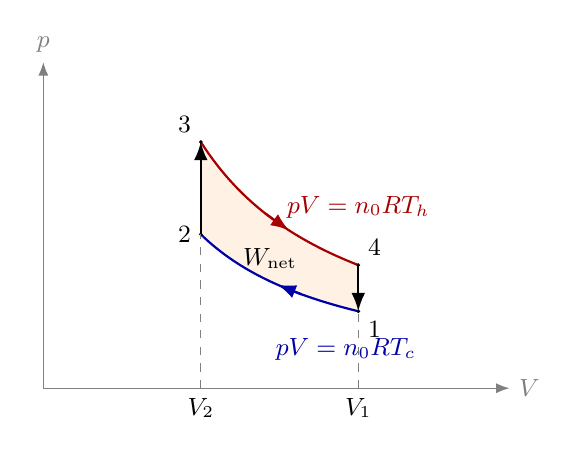
\begin{tikzpicture}[font=\small,x=1.6cm,y=1.15cm]
\draw[->,gray](0,0)--(3.7,0)node[right]{$V$};
\draw[->,gray](0,0)--(0,3.6)node[above]{$p$};
\fill[orange!10,domain=1.25:2.5,samples=100]
 (1.25,2.72)--plot(\x,{3.4/\x})--(2.5,.85)--plot[domain=2.5:1.25](\x,{2.125/\x})--cycle;
\draw[blue!65!black,thick,domain=1.25:2.5,samples=100]plot(\x,{2.125/\x});
\draw[red!65!black,thick,domain=1.25:2.5,samples=100]plot(\x,{3.4/\x});
\draw[thick,->](1.25,1.7)--(1.25,2.72);
\draw[thick,->](2.5,1.36)--(2.5,.85);
\draw[blue!65!black,thick,->](2.05,{2.125/2.05})--(1.86,{2.125/1.86});
\draw[red!65!black,thick,->](1.76,{3.4/1.76})--(1.95,{3.4/1.95});
\foreach \xx/\yy/\num/\pos in {2.5/.85/1/below right,1.25/1.7/2/left,1.25/2.72/3/above left,2.5/1.36/4/above right}{
 \fill(\xx,\yy)circle[radius=.025cm]node[\pos]{$\num$};}
\draw[gray,dashed](1.25,0)--(1.25,1.7);\draw[gray,dashed](2.5,0)--(2.5,.85);
\node[below]at(1.25,0){$V_2$};\node[below]at(2.5,0){$V_1$};
\node[hot]at(2.5,2.0){$pV=n_0RT_h$};
\node[cold]at(2.4,.43){$pV=n_0RT_c$};
\node at(1.8,1.43){$W_{\rm net}$};
\end{tikzpicture}
\begin{tikzpicture}[font=\small]
\filldraw[fill=red!8](-3.25,-.65)rectangle(-.17,.65);
\filldraw[fill=blue!8](.17,-.65)rectangle(1.7,.65);
\filldraw[pattern=north east lines](-.17,-.65)rectangle(.17,.65);
\fill[gray!50](-3.38,-.65)rectangle(-3.25,.65);
\fill[gray!50](1.7,-.65)rectangle(1.83,.65);
\node[hot,align=center]at(-1.7,0){$T_h$\\[2pt]$n_h=n_0/2$};
\node[cold,align=center]at(.95,0){$T_c$\\[2pt]$n_c=n_0/2$};
\draw[heat](-1.7,1.35)--(-1.7,.68)node[pos=0,above]{$\delta Q_h$};
\draw[heat](.95,.68)--(.95,1.35)node[pos=1,above]{$-\delta Q_c$};
\draw[blue!65!black,thick,->](.55,.86)--(-.55,.86);
\node[below]at(0,-1.4){同一压力 $p$，两腔温度不同};
\draw[<->,gray](-3.25,-.95)--(-.17,-.95)node[midway,below,text=black]{$V_h$};
\draw[<->,gray](.17,-.95)--(1.7,-.95)node[midway,below,text=black]{$V_c$};
\end{tikzpicture}
\begin{tikzpicture}[font=\small]
\foreach \shift/\stage in {0/{2\to3},6.8/{4\to1}}{
\begin{scope}[xshift=\shift cm]
\node[draw,fill=red!8,minimum width=4.1cm,minimum height=.6cm]at(0,2){高温热源 $T_h$};
\node[draw,fill=gray!5,minimum width=4.1cm,minimum height=.8cm]at(0,0){两腔气体：$\stage$};
\node[draw,fill=blue!8,minimum width=4.1cm,minimum height=.6cm]at(0,-2){低温热源 $T_c$};
\draw[heat](0,1.65)--(0,.45);
\draw[heat](0,-.45)--(0,-1.65);
\end{scope}
}
\node[right]at(.18,1){$Q_{h,2}>0$};
\node[right]at(.18,-1){$-Q_{c,2}>0$};
\node[right]at(6.98,1){$Q_{h,4}>0$};
\node[right]at(6.98,-1){$-Q_{c,4}>0$};
\node[below]at(3.4,-2.65){无储热多孔塞模型；热源供热不等于两腔净吸热};
\end{tikzpicture}
\end{document}
